% 第三章

\chapter{移植PKE的总体设计}

\section{移植PKE到K210的背景}

接下来,本文将通过阐述PKE移植前的开发环境与移植后的预期收益,
介绍移植PKE到K210的背景。

\subsection{PKE移植前开发环境介绍}

PKE移植前的运行环境主要分为两种,分别是硬件环境和模拟器环境。
他们的总体情况是一致的,但还是有一些细微的区别。

在模拟器环境上,PKE运行在spike模拟的RISC-V 64位机器上。
而spike模拟器则运行在宿主机Ubuntu上。
当PKE需要使用外部设备的I/O功能时,
PKE就通过调用spike提供的HTIF接口,
让Ubuntu提供I/O功能,以访问宿主机上的外设资源。

如下图,本文给出了模拟器环境的系统架构。

\begin{figure}[htbp]
    \vspace{13pt} % 调整图片与上文的垂直距离
    \centering
    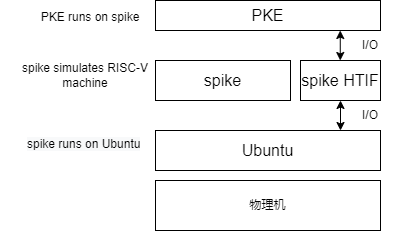
\includegraphics[width=0.6\textwidth]{images/spike_structure.png}
    \caption{模拟器环境架构}\label{模拟器环境架构} % label 用来在文中索引
\end{figure}

在硬件环境上,我们的系统是运行上PYNQ-Z2开发板上。
PYNQ-Z2开发板是Xilinx公司的一款开发板,
它具有丰富的外设资源、强大的性能。此外,它还兼容了Arduino和树莓派接口。

PYNQ-Z2搭载了FPGA系统和ARM处理器。FPGA可以烧录RISC-V CPU软核,
ARM硬核可以运行Ubuntu操作系统。我们的代理内核PKE运行在RISC-V CPU软核上,
而提供外设功能的Ubuntu则运行在ARM硬核上。
PKE和Ubuntu之间是通过riscv-fesvr通信的。
riscv-fesvr是PYNQ开发板上的重要工具,没有它,PKE就无法调用ARM上的Ubuntu I/O接口。
riscv-fesvr通过共享内存的方式,接收PKE的请求,使用ARM端的资源,并向PKE提供资源与功能。

如下图,本文给出了硬件环境的系统架构。

\begin{figure}[htbp]
    \vspace{13pt} % 调整图片与上文的垂直距离
    \centering
    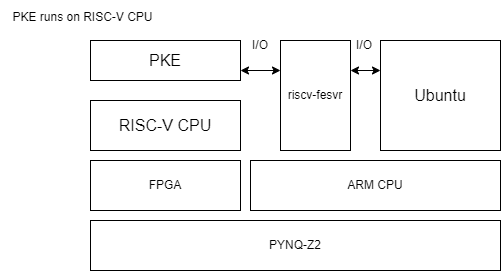
\includegraphics[width=0.6\textwidth]{images/pke_hardware_env.drawio.png}
    \caption{硬件环境架构}\label{硬件环境架构} % label 用来在文中索引
\end{figure}

\subsection{PKE移植前开发环境的优缺点}

在上一小节,本文简单介绍了PKE在移植前的开发环境。
在本小节,本文会客观分析PKE原先的物理开发环境的优点与缺点。

在原先的物理环境中,代理内核的系统是运行在PYNQ-Z2板子上的。
PYNQ-Z2拥有FPGA和ARM物理核。FPGA可以让开发者烧录RISC-V CPU软核,
然后让开发者在RISC-V CPU软核上运行PKE。
ARM硬核可以运行Ubuntu操作系统,提供I/O功能。

从不同的开发方向看。
如果开发者是在开发CPU软核,
需要快速验证FPGA上的CPU软核并进行迭代。
这种物理环境允许开发者不实现CPU涉及I/O的功能,
便于开发快速开发和验证CPU软核。

如果开发者是在开发或学习操作系统,这种开发环境反而对开发者不利。
一个原因是提供这种物理环境的开发板PYNQ-Z2价格昂贵,成本高昂。
其价格已经快要接近一台PC机的价格。
此开发板在某网购平台上的均价已达到三千余元。
这对入门级操作系统学习者购买资料学习、课程实验教学都是不利的。

另一个原因环境配置繁琐,开发者需要在PYNQ上烧录RISC-V CPU软核,
还需要在ARM核上部署Ubuntu。
除此之外,还需要在ARM核上部署riscv-fesvr,让PKE与Ubuntu通信。
这种开发环境的部署成本和学习成本是很高的,
这对于刚入门操作系统实验学习的开发者是不利的。

总而言之,PKE系统的物理环境价格昂贵、成本高昂、搭建成本高、学习成本高,
不利于学习者入门,也不利于大规模展开实验教学。
这些是PKE移植前的物理环境的痛点。
为了解决这些痛点,本文提出了将PKE移植到K210上的方案。将在下一小节阐述该方案的收益。

\subsection{PKE移植后的预期收益}

上一小节我们提到,PKE原先的物理环境有许多缺点。
这些缺点不利于学习者入门、也不利于大规模展开实验教学。
因此,我们计划将PKE移植到K210物理环境上。
PKE移植后,我们将拥有如下收益:

\begin{enumerate}
    \item 成本低廉
    
    K210板子价格低廉。
    一块不带外设的普通K210 SoC的市场价格只需要一百多元。
    与动则就要三千余元的PYNQ-Z2相比,K210的经济成本仅仅是PYNQ-Z2的三十分之一。
    这非常有利于我们开展大规模的物理环境实验教学。
    也非常有利于入门学习者购买资料进行学习。

    \item 物理环境搭建成本低
    
    在K210上,我们不再像从前在PYNQ-Z2那样烧录RISC-V CPU软核,
    也不需要在PYNQ-Z2的ARM核上加载运行Ubuntu。
    由于K210带有RISC-V 64位CPU,我们只需要在K210上烧录并运行PKE即可。
    这使得我们的物理环境搭建成本变得极低。

    \item 环境搭建学习成本低
    
    移植PKE到K210后,我们可以使用docker配置环境包、
    编写Makefile将编译与烧录流程变得自动化。
    由于不再需要像在PYNQ-Z2上烧录RISC-V CPU软核,
    也不需要在PYNQ-Z2的ARM核上加载运行Ubuntu。
    我们的环境搭建是自动化的。环境搭建的学习成本也是很低的。

\end{enumerate}


\section{移植PKE的目标与需求分析}

\begin{enumerate}

    \item 降低PKE在物理环境的开发成本
    
    移植PKE的首要目标,是降低PKE在物理环境的开发成本。
    这其中包括降低购买硬件资源的经济成本,也包括降低环境搭建的学习成本。
    这将有利于我们后续开展大规模的物理环境实验。
    也会有利于降低PKE实验的学习门槛。

    \item 用户态程序无感知
    
    PKE在移植K210的过程中,会有一定程度的内核态代码修改。
    从实验迁移的角度来看,这些内核态代码的修改应该让用户态程序无感知。
    否则,我们很有可能还要修改用户态程序,以适配修改过的PKE。
    这不仅会增加我们移植PKE的开发成本,也会增加后续实验操作者的学习成本。

    \item 减少实验操作者对移植的感知
    
    PKE移植后产生的内核态代码修改,应该尽可能地不让实验操作者感知。
    修改过后的PKE,应该对实验操作者提供与原先一致的接口,
    以降低移植对实验操作者的影响。

    \item 提高实验操作者的开发效率
    
    移植后的PKE需要能做到提高实验操作者的开发效率,
    如环境搭建更加简化、编译流程和烧录流程更加自动化、
    调试过程更加清晰化、提供给实验者的API更加易用。
    
    \item 降低PKE后续移植的成本

    经过改造后的PKE,后续移植到其他RISC-V开发板时,它的移植成本应该降低。
    也就是说,我们的移植工作应该是可复用的。
    只要是将PKE移植到其他的RISC-V开发板,我们都应该尽可能地减少对内核代码的改动。
    
\end{enumerate}

\section{移植K210前PKE的总体设计}

\subsection{系统架构}

\subsection{主要功能模块介绍}

\subsection{执行流程}

\section{移植PKE到K210的技术方案}

\section{移植K210后PKE的总体设计}

\subsection{系统架构}

\subsection{主要功能模块介绍}

\subsection{执行流程}
你好
